We consider a traffic signal control application where the aim is to improve the road user experience by an adaptive traffic light control (TLC) algorithm.
We adopt a CPT approach, i.e., apply the CPT-functional to the delay experienced by road users. We then optimize the CPT-value of the delay  and contrast this approach with a traditional expected delay optimizing algorithm.

\subsection{Simulation Setup}  
Consider a road network with $\N$ signalled lanes that are spread across junctions and $\M$ paths, where each path connects (uniquely) two edge nodes, where the traffic is generated - see Figure \ref{fig:2x2grid}.
At any instant $n$, let $q_n^i$ and $t_n^i$ denote the queue length and elapsed time since the lane turned red, for any lane $i = 1,\ldots, \N$. Let $d_n^{i,j}$ denote the delay experienced by $j$th road user on $i$th path, for any $i=1,\ldots,\M$ and $j=1,\ldots,n_i$, where $n_i$ denotes the number of road users on path $i$.
We specify the various components of the traffic control MDP in the following.
The state $s_n=(q_n^1,\ldots,q_n^{\N},t_n^1,\ldots,t_n^{\N},d_n^{1,1},\ldots,d_n^{\M,n_{\M}})\tr$ is a vector of lane-wise queue lengths, elapsed times and path-wise delays.
The actions are the feasible sign configurations that specify red-green combinations for the traffic lights in the road network considered. 
The return is defined as follows:
  


The weights and utilities in \eqref{eq:cpt-general} are chosen as follows:
\begin{align*}
w^+(p) = &\frac{p^{\eta_1}}{{(p^{\eta_1}+ (1-p)^{\eta_1})}^{1/\eta_1}}, \\
w^-(p) =& \frac{p^{\eta_2}}{{(p^{\eta_2}+ (1-p)^{\eta_2})}^{1/\eta_2}},\\
u^+(x) = & |x|^{\sigma}, \text{ and }  u^-(x) = \lambda |x|^{\sigma},
\end{align*}
where we set $\eta_1 = 0.61$, $\eta_2 = 0.69$, $\lambda = 2.25$ and $\sigma = 0.88$. These choices are based on median estimates given by \cite{tversky1992advances} and have been employed earlier in a traffic application in \cite{gao2010adaptive}.
 
\begin{figure}
\centering
        \includegraphics[width=2.2in,height=1.5in]{fig/2x2grid.pdf}
  \caption{The 2x2-grid network used in our experiments.}
\label{fig:2x2grid}
  \end{figure}


 \begin{figure}[t]
    \centering
     \begin{tabular}{cc}
\subfigure[AVG-SPSA]{
\label{fig:runtimes}
%\hspace{2em} 
\tabl{c}{\scalebox{0.7}{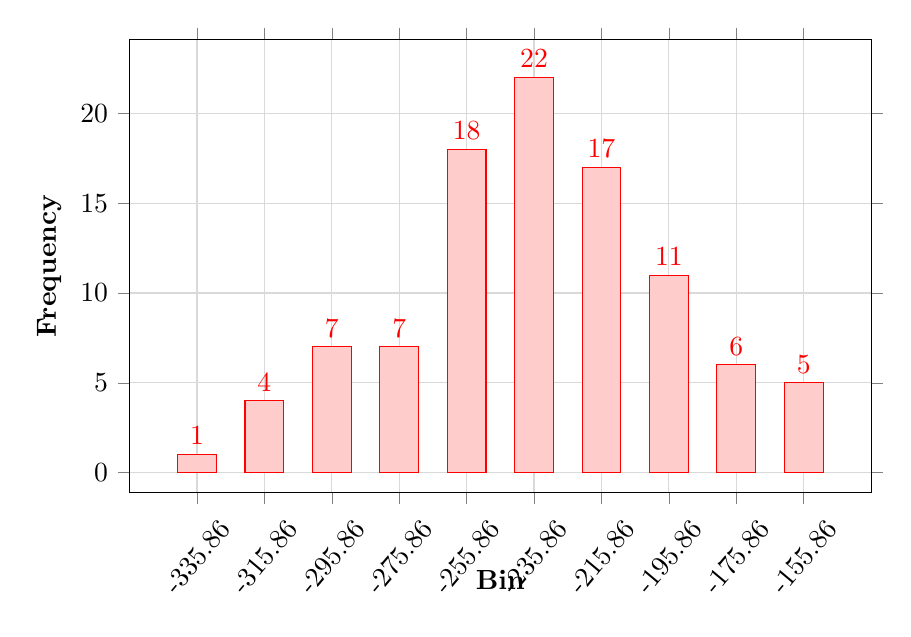
\begin{tikzpicture}
\begin{axis}[
ybar={2pt},
%  legend style={at={(0.5,-0.2)},anchor=north,legend columns=-1},
legend pos=outer north east,
legend image code/.code={\path[fill=white,white] (-2mm,-2mm) rectangle
(-3mm,2mm); \path[fill=white,white] (-2mm,-2mm) rectangle (2mm,-3mm); \draw
(-2mm,-2mm) rectangle (2mm,2mm);},
ylabel={\bf Frequency},
xlabel={\textbf{Bin}},
x label style={at={(axis description cs:0.5,-0.15)},anchor=north},
symbolic x coords={0, -335.86, -315.86, -295.86, -275.86, -255.86, -235.86, -215.86, -195.86, -175.86, -155.86, 11},
xmin={0},
xmax={11},
xtick=data,
ytick align=outside,
%xticklabels={{\bf7x9-Grid\\[0.5ex]($d=504$),\bf 14x9-Grid\\[0.5ex]($d=1008$),\bf 14x18-Grid\\[0.5ex]($d=2016$),\bf 28x18-Grid\\[0.5ex]($d=4032$)}},
xticklabel style={rotate=50, align=center},
bar width=14pt,
nodes near coords,
grid,
grid style={gray!30},
width=11cm,
height=7.33cm,
]
\addplot[red, fill=red!20]   coordinates {  (-335.86,1) (-315.86,4) (-295.86,7) (-275.86,7) (-255.86,18) (-235.86,22) (-215.86,17) (-195.86,11) (-175.86,6) (-155.86,5)}; %LSPI
\end{axis}
\end{tikzpicture}}\\[1ex]}
}
\\
%%%%%%%%%%%%%%
\subfigure[EUT-SPSA]{
\label{fig:runtimes}
%\hspace{2em} 
\tabl{c}{\scalebox{0.7}{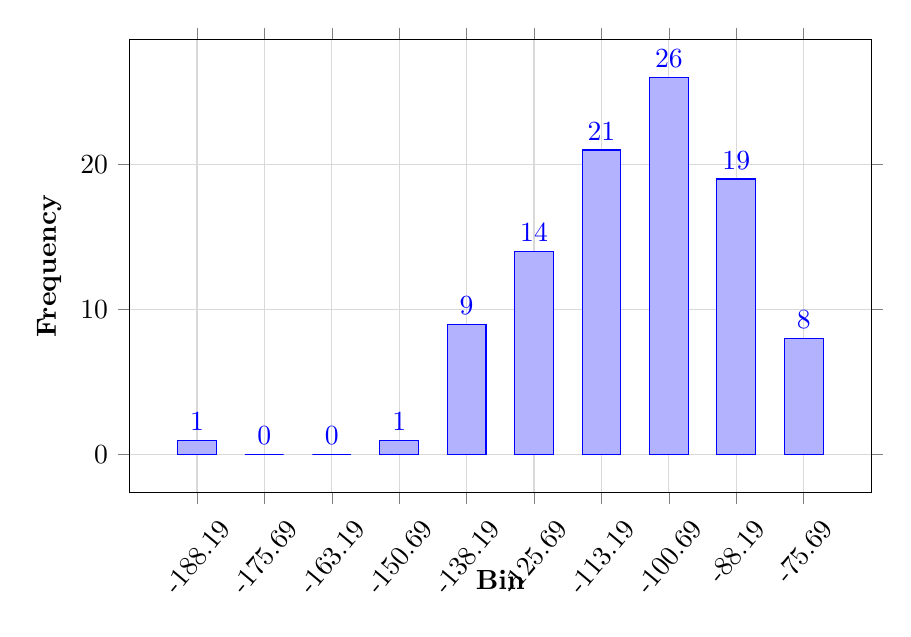
\begin{tikzpicture}
\begin{axis}[
ybar={2pt},
%  legend style={at={(0.5,-0.2)},anchor=north,legend columns=-1},
legend pos=outer north east,
legend image code/.code={\path[fill=white,white] (-2mm,-2mm) rectangle
(-3mm,2mm); \path[fill=white,white] (-2mm,-2mm) rectangle (2mm,-3mm); \draw
(-2mm,-2mm) rectangle (2mm,2mm);},
ylabel={\bf Frequency},
xlabel={\textbf{Bin}},
x label style={at={(axis description cs:0.5,-0.15)},anchor=north},
symbolic x coords={0,-188.19,-175.69,-163.19,-150.69,-138.19,-125.69,-113.19,-100.69,-88.19,-75.69,11},
xmin={0},
xmax={11},
xtick=data,
ytick align=outside,
%xticklabels={{\bf7x9-Grid\\[0.5ex]($d=504$),\bf 14x9-Grid\\[0.5ex]($d=1008$),\bf 14x18-Grid\\[0.5ex]($d=2016$),\bf 28x18-Grid\\[0.5ex]($d=4032$)}},
xticklabel style={rotate=50, align=center},
bar width=14pt,
nodes near coords,
grid,
grid style={gray!30},
width=11cm,
height=7.33cm,
]
\addplot   coordinates {  (-188.19,1) (-175.69,0) (-163.19,0) (-150.69,1) (-138.19,9) (-125.69,14) (-113.19,21) (-100.69,26) (-88.19,19) (-75.69,8) }; %LSPI
\end{axis}
\end{tikzpicture}}\\[1ex]}
}
\\
%%%%%%%%%%%%%%%%%%%%%%%%%
\subfigure[CPT-SPSA]{
\label{fig:runtimes}
%\hspace{2em} 
\tabl{c}{\scalebox{0.7}{\begin{tikzpicture}
\begin{axis}[
ybar={2pt},
%  legend style={at={(0.5,-0.2)},anchor=north,legend columns=-1},
legend pos=outer north east,
legend image code/.code={\path[fill=white,white] (-2mm,-2mm) rectangle
(-3mm,2mm); \path[fill=white,white] (-2mm,-2mm) rectangle (2mm,-3mm); \draw
(-2mm,-2mm) rectangle (2mm,2mm);},
ylabel={\bf Frequency},
xlabel={\textbf{Bin}},
x label style={at={(axis description cs:0.5,-0.15)},anchor=north},
symbolic x coords={0, -43.36,-33.36,-23.36,-13.36,-3.36,6.64,16.64,26.64,36.64,46.64, 11},
xmin={0},
xmax={11},
xtick=data,
ytick align=outside,
%xticklabels={{\bf7x9-Grid\\[0.5ex]($d=504$),\bf 14x9-Grid\\[0.5ex]($d=1008$),\bf 14x18-Grid\\[0.5ex]($d=2016$),\bf 28x18-Grid\\[0.5ex]($d=4032$)}},
xticklabel style={rotate=50, align=center},
bar width=14pt,
nodes near coords,
grid,
grid style={gray!30},
width=11cm,
height=7.33cm,
]
\addplot[darkgreen, fill=darkgreen!20]   coordinates {  (-43.36,1) (-33.36,0) (-23.36,0) (-13.36,1) (-3.36,0) (6.64,1) (16.64,8) (26.64,52) (36.64,24) (46.64,12) }; %LSPI
\end{axis}
\end{tikzpicture}}\\[1ex]}
}
\end{tabular}
\caption{Histogram of CPT-value of the average delay for four different algorithms}
\label{fig:normdiff-perf}
\end{figure}

%We consider a SSP version of an example\footnote{A similar example has been considered in \cite{chow2014algorithms}.} for buying a house at the optimal price. Suppose the house is priced at $x_k$ at any instant $k$ and at the next instant, the price either goes down to $\left(x_k \times C_{down}\right)$ w.p. $p_{down}$ or goes up to $\left(x_k\times C_{up}\right)$ w.p. $1-p_{down}$. The actions are to either wait (denoted $w$), which results in a holding cost $h$ or to buy (denoted $b$) at the current price. The horizon is capped at $T$, with a terminal cost $x_T$.  The goal is to minimize the total cost defined as $ 
%D^{\theta}(x^0)= \sum_{k=0}^\tau \left(I_{\{a_k =b \} }x_k+I_{\{a_k =w \} } h\right) + I_{\{\tau=T\}} x_T$, where $\tau =  \{k | \theta(x_k)=1 \} \wedge T$.
%We set $T=20, h=0.1, C_{up}=2, C_{down}=0.5$, and $x_0=1$.  
%
 %\begin{figure*}
    %\centering
     %\begin{tabular}{cc}
%\begin{subfigure}[b]{0.5\textwidth}
%\tabl{c}{\scalebox{0.7}{\begin{tikzpicture}
%\begin{axis}[
%ybar={2pt},
%legend pos=north east,
%legend image code/.code={\path[fill=white,white] (-2mm,-2mm) rectangle
%(-3mm,2mm); \path[fill=white,white] (-2mm,-2mm) rectangle (2mm,-3mm); \draw
%(-2mm,-2mm) rectangle (2mm,2mm);},
%ylabel={\bf Expected value},
%xlabel={\bf Probability $\bm{p_{down}}$},
%xtick=data,
%ytick align=outside,
%xticklabel style={align=center},
%ymin=0.1,
%ymax=1.4,
%bar width=14pt,
%nodes near coords,
%grid,
%grid style={gray!30},
%width=11cm,
%height=9.5cm,
%]
%\addplot[fill=red!20]  table[x index=0, y index=1, col sep=comma] {../results/Valueiteration.txt} ;
%\addlegendentry{Value iteration}
%\end{axis}
%\end{tikzpicture}}\\[1ex]}
%\caption{Value iteration}
%\label{fig:vi}
%\end{subfigure}
%&
%\begin{subfigure}[b]{0.5\textwidth}
%\tabl{c}{\scalebox{0.7}{\begin{tikzpicture}
%\begin{axis}[
%ybar={2pt},
%legend pos=north east,
%legend image code/.code={\path[fill=white,white] (-2mm,-2mm) rectangle
%(-3mm,2mm); \path[fill=white,white] (-2mm,-2mm) rectangle (2mm,-3mm); \draw
%(-2mm,-2mm) rectangle (2mm,2mm);},
%ylabel={\bf CPT-Value},
%xlabel={\bf Probability $\bm{p_{down}}$},
%xtick=data,
%ytick align=outside,
%xticklabel style={align=center},
%bar width=14pt,
%ymin=0.1,
%ymax=1.4,
%nodes near coords,
%grid,
%grid style={gray!30},
%width=11cm,
%height=9.5cm,
%]
%\addplot[fill=blue!20]  table[x index=0, y index=1, col sep=comma] {../results/twospsa_cpt.txt} ;
%\addlegendentry{CPT-SPSA-N}
%\end{axis}
%\end{tikzpicture}}\\[1ex]}
%\caption{Second-order SPSA for CPT-value}
%\label{fig:cpt2spsa}
%\end{subfigure}
%\\
%\begin{subfigure}[b]{0.5\textwidth}
    %\tabl{c}{\scalebox{0.7}{\begin{tikzpicture}
%\begin{axis}[
%ybar={2pt},
%legend pos=north east,
%legend image code/.code={\path[fill=white,white] (-2mm,-2mm) rectangle
%(-3mm,2mm); \path[fill=white,white] (-2mm,-2mm) rectangle (2mm,-3mm); \draw
%(-2mm,-2mm) rectangle (2mm,2mm);},
%ylabel={\bf Expected value},
%xlabel={\bf Probability $\bm{p_{down}}$},
%xtick=data,
%ytick align=outside,
%xticklabel style={align=center},
%ymin=0.1,
%ymax=1.8,
%bar width=14pt,
%nodes near coords,
%grid,
%grid style={gray!30},
%width=11cm,
%height=9.5cm,
%]
%\addplot[fill=yellow!30]  table[x index=0, y index=1, col sep=comma] {../results/SPSADETERMINISTIC.txt} ;
%\addlegendentry{NoCPT-SPSA-G}
%\end{axis}
%\end{tikzpicture}}\\[1ex]}
%\caption{SPSA for regular value function}
%\label{fig:nocptspsa}
%\end{subfigure}
%&
%\begin{subfigure}[b]{0.5\textwidth}
%\tabl{c}{\scalebox{0.7}{\begin{tikzpicture}
%\begin{axis}[
%ybar={2pt},
%legend pos=north east,
%legend image code/.code={\path[fill=white,white] (-2mm,-2mm) rectangle
%(-3mm,2mm); \path[fill=white,white] (-2mm,-2mm) rectangle (2mm,-3mm); \draw
%(-2mm,-2mm) rectangle (2mm,2mm);},
%ylabel={\bf CPT-Value},
%xlabel={\bf Probability $\bm{p_{down}}$},
%xtick=data,
%ytick align=outside,
%xticklabel style={align=center},
%bar width=14pt,
%ymin=0.1,
%ymax=1.4,
%nodes near coords,
%grid,
%grid style={gray!30},
%width=11cm,
%height=9.5cm,
%]
%\addplot[fill=green!20]  table[x index=0, y index=1, col sep=comma] {../results/SPSACPT.txt} ;
%\addlegendentry{CPT-SPSA-G}
%\end{axis}
%\end{tikzpicture}}\\[1ex]}
%\caption{First-order SPSA for CPT-value}
%\label{fig:cptspsa}
%\end{subfigure}
%\end{tabular}
%\caption{Performance of policy gradient algorithms with/without CPT for different down probabilities of the SSP}
%\label{fig:perf}
%\end{figure*}
%
%
  %
%
%\paragraph{Implementation:} On this example, we implement the first-order CPT-SPSA-G and the second-order CPT-SPSA-N algorithms. For the sake of comparison, we also apply value iteration to the SSP example described above. 
%Note that value iteration requires knowledge of the model, while our CPT based algorithms estimate CPT-value using simulated episodes.
%We implement the algorithm from \cite{bhatnagar2004simultaneous} for the SSP example described in the numerical experiments of the main paper. The latter, henceforth referred to as NoCPT-SPSA-G, is an SPSA-based scheme that optimizes the traditional value function objective in a discounted MDP setting and we make a trivial adaptation of this algorithm for the SSP setting.
%For CPT-SPSA-G and NoCPT-SPSA-G, we set $\delta_n = 1.9/n^{0.101}$ and $\gamma_n = 1/n$, while for CPT-SPSA-N, we set $\delta_n=3.8/n^{0.166}$ and $\gamma_n=1/n^{0.6}$. For all algorithms, we set each entry of the initial policy $\theta_0$ to $0.1$. For CPT-value estimation, we simulate $1000$ SSP episodes, with the SSP horizon $T$ set to $20$. All algorithms are run with a budget of $1000$ samples, which implies $500$ iterations of CPT-SPSA-G and $333$ iterations of CPT-SPSA-N. The results presented are averages over $500$ independent simulations. For CPT-SPSA-G/CPT-SPSA-N, 
%the weight functions $w^+$ and $w^-$ are set to $p^{0.6}/(p^{0.6}+(1-p)^{0.6})$, while the utility functions are identity maps. 
%
%
%
%\subsection{Results} Figures \ref{fig:vi}--\ref{fig:nocptspsa} present the value function computed using value iteration and NoCPT-SPSA-G, while Figures \ref{fig:cptspsa}--\ref{fig:cpt2spsa} present the CPT-value $V^{\theta_{end}}(x^0)$ for CPT-SPSA-G and CPT-SPSA-N, respectively. The performance plots are for various values of $p_{down}$, the probability of house price going down. 
%From Figure \ref{fig:vi}, we notice that the variations in expected total cost is larger in comparison to that in CPT-value. Figure \ref{fig:nocptspsa} implies that a similar observation about variation of expected value holds true for NoCPT-SPSA-G algorithm from \cite{bhatnagar2004simultaneous}. While it is difficult to plot the entire policies, for the expected value minimizing algorithms it was observed that there were drastic changes in the policies with a change of $0.01$ in $p_{down}$, while PG/CPT-SPSA-N resulted in randomized policies that smoothly transitioned with changes in $p_{down}$.
%As motivated in the introduction, these plots verify that CPT-aware SPSA algorithms are less sensitive to the model changes as compared to the expected value minimizing algorithms. It is also evident that the second-order CPT-SPSA-N gives marginally better results than its first-order counterpart CPT-SPSA-G.
 %Finally, what is not shown is that the CPT-value obtained for PG/CPT-SPSA-N is much lower than that obtained for NoCPT-SPSA-G, thus making apparent the need for specialized algorithms that incorporate CPT-based criteria.
%
